\documentclass{article}

% Language setting
% Replace `english' with e.g. `spanish' to change the document language
\usepackage[english]{babel}

% Set page size and margins
% Replace `letterpaper' with `a4paper' for UK/EU standard size
\usepackage[letterpaper,top=2cm,bottom=2cm,left=3cm,right=3cm,marginparwidth=1.75cm]{geometry}

% Useful packages
\usepackage[utf8]{inputenc}
\usepackage{amsmath}
\usepackage{graphicx}
\usepackage[colorlinks=true, allcolors=blue]{hyperref}

\usepackage[style=apa, backend=biber]{biblatex}
\DefineBibliographyStrings{english}{%
  bibliography = {References},
}

\usepackage{caption}

\addbibresource{refs.bib}


\title{An Overview of Java Web Programming}
\author{Matthew Robinson}

\usepackage{CJKutf8}
\begin{document}
\begin{CJK}{UTF8}{gbsn}
\maketitle

\begin{abstract}
This paper proposes a new approach to optimise blockchain ledger sizes along a network by using multi-level caching in order to reduce the ledger sizes on the nodes.
\end{abstract}

\tableofcontents
\listoffigures

\section{Introduction}
Blockchain technology has revolutionised the way we store and transfer data, providing a secure and decentralised ledger that is transparent and tamper-proof. However, current methods are inefficient, as they require nodes to store and retrieve large amounts of data (S.Zhi-Xin, Z.Xin, X. Feng, C. Lu, 2021) . This is particularly true for the Bitcoin blockchain, where all users must have a complete clone of the ledger, even though only a small portion of the blocks will be needed for most users at any given time. As such, there is a need to explore more efficient methods for utilizing blockchain technology to ensure that it remains a viable option for storing and transferring data in the years to come.

\section{Problem Statement/Aim and Objectives}

Problem: The problem this research will investigate is potential methods in decreasing block duplication in order to reduce total storage usage in a distributed blockchain network.\\

Aim: The aim of this experiment is to develop a protocol and topology to overcome the drawback of a typical blockchain storage duplication issues whilst still maintaining strong availability and security.


\section{Background}

There are numerous theories and implementations to decrease the storage size of distributed ledgers. An implementation of the blockchain ledger would be in the use of cryptocurrencies. For example; in popular currency Bitcoin, the ledger contains information such as transaction receipts, addresses, timestamps, etc. According to bitcoinist, 78\% of supply is in long term holders accounts (Hououin Kyouma,2023). This means that under a quarter of wallets are touched and thus transactions that are rarely accessed. In this circumstance the majority of users wouldn’t need this infrequently used ledger data duplicated on their machines. This would be a appropriate use of the proposed model because it would solve a core underlying problem.

\noindent\makebox[\textwidth]{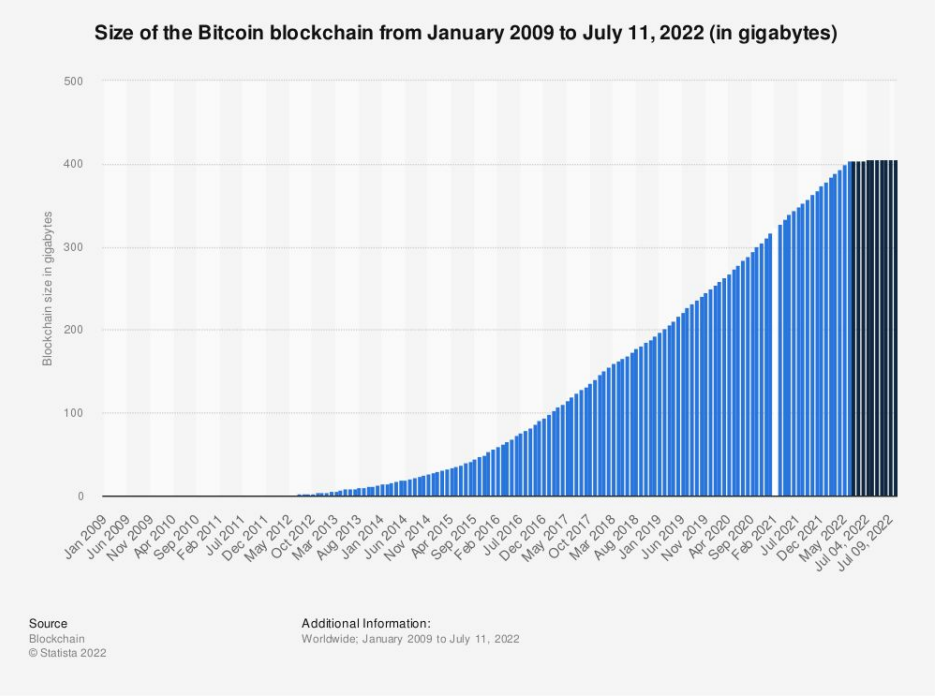
\includegraphics[width=\textwidth]{stastica.PNG}}
\captionof{figure}{Increase in ledger size per year}

Another similar implementation would be the InterPlanetary File System (IPFS). A decentralized file system that employs a distributed hash table (DHT) and the Kademlia algorithm to search through distributed node DHTs in O(log(n)) time (IPFS, 2023) . Although this is not inherently “blockchain” by definition. In many ways a DHT is similar to a ledger in the sense it provides hashed information to the user and holds duplicate information amongst distributed nodes. To prevent DHT sizes from becoming too large, every node maintains a partial DHT. For example, a network with 10,000,000 nodes would take 23 hops on average to get to the destination. With a centralized network, an average number of hops a user browsing makes can greatly depend on a number of factors such as the user’s location, network infrastructure and complexity of the website being accessed.

\noindent\makebox[\textwidth]{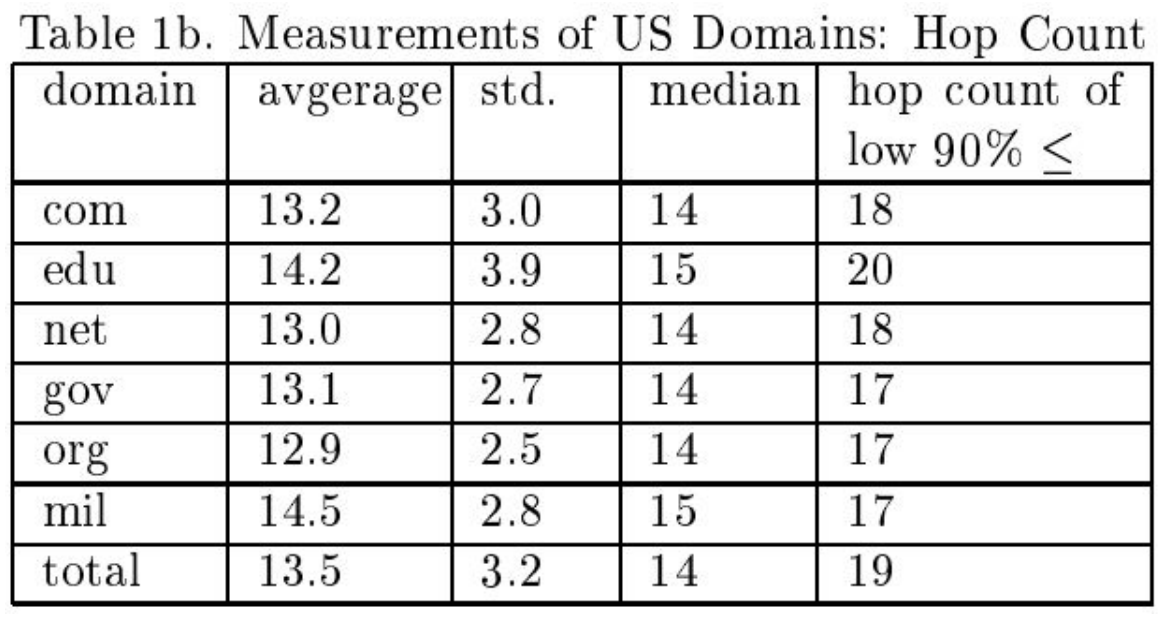
\includegraphics[width=\textwidth]{hopcount.PNG}}
\captionof{figure}{Average hop counts in a centralised network}

However in the following article it cites that the average users browsing activity is between 10-20 network hops Fei, A., Pei, G., \& Liu, R,  2013) . IPFS implementation doesn’t require a significant increase in hops in comparison to standard usage. A limitation of the IPFS protocol is that it doesn’t ensure availability as there is no incentive for users to download and share content. This method of partial DHT files could be implemented into the blockchain ledger. whilst maintaining a few central nodes holding the entire ledger in order  to ensure availability.

\section{Experimental Design}

Aim: Design a proof of concept protocol which reduces infrequently accessed blocks by introducing a frequency counter in a blockchain network. Develop a class based system which labels the nodes based on reliability. High reliability nodes will have all data whereas the less reliable nodes will act as a cache, holding the most frequently accessed blocks. An implementation of the system will be evaluated and compared to traditional storage methods, demonstrating its effectiveness in improving blockchain storage efficiency.\\

Hypothesis: After getting the total file sizes of each node, I estimate that the total file size across all nodes will be significantly smaller than the original method. \\

Control Variable: Number of nodes on the network will remain the same. As well as the total unique data content.\\

Method: I will simulate a distributed network by setting up a collection of nodes on a network class and assign them random lifespan values. The protocol will enable them to communicate with each-other and assign themselves a stability value (SV) based on their lifespans. The lower SV’s will hold less data but more frequently accessed whereas the highest class will hold the entire ledger. These nodes will be arranged in a cluster of 4 where each node has a different SV. Once a node joins the network, it will query whether a cluster needs it. If not, it will start it’s own cluster and clone the ledger information from the nearest NC of the same class or higher.\\

My dependent variable will be the total storage across all nodes whereas the independent variable will be the distribution protocol.

\section{Results}
As you can see from the results of figure 3 and 4, as the number of blocks increases. So does the overall network size. However, utilising the caching, the overall redundancy of the network is half the size. 

\noindent\makebox[\textwidth]{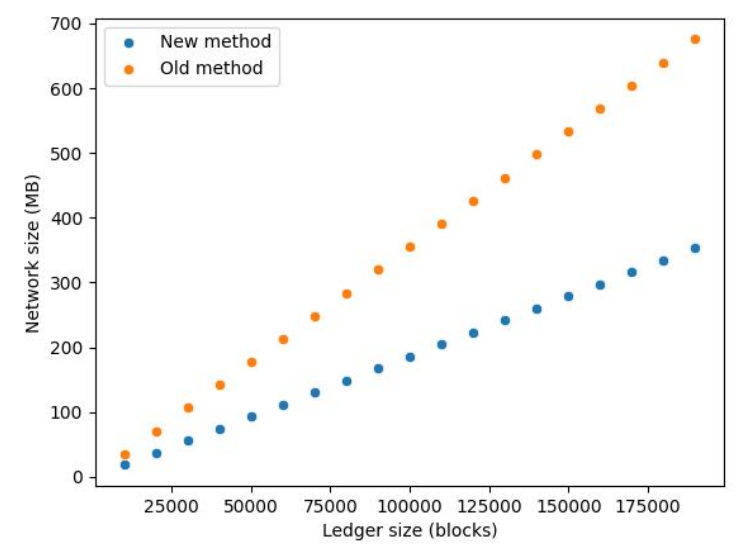
\includegraphics[width=\textwidth]{ledger1.PNG}}
\captionof{figure}{Large ledger}

As you can see from figure 4, the size of the ledger is irrelevant. The new model with the current parameters will always result in a 50\% replication reduction in the network.

\noindent\makebox[\textwidth]{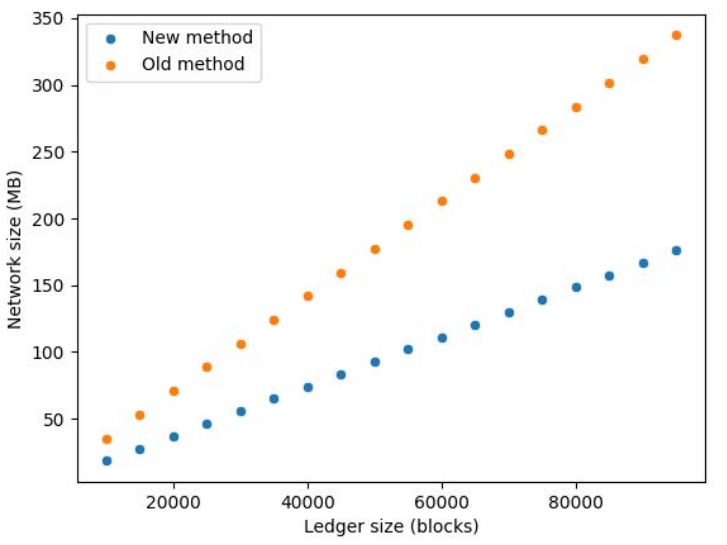
\includegraphics[width=\textwidth]{ledger2.PNG}}
\captionof{figure}{Small ledger}

However, this may come at the expense latency from the increased number of server hops when accessing infrequently accessed blocks.

\section{Discussion}
In this simulation, the clusters are broken into groups of four. Each of which is assigned a SV of; weakest, weak, strong, strongest based on their network longevity. Holding ¼, ½, ¾,1 of the frequently sorted blocks respectively.\\

In the diagram you can see that at 190,000 blocks, the old method had a network total of 270MB across all nodes whereas the new method only had 140MB total. This is a significant improvement. Depending on the parameters of the simulation and the implementation, the majority of nodes could have the ability of having ledger size reduced further.\\

Additionally, the protocol arranges the nodes in a way that prioritizes recently accessed nodes, which reflects a real-world popularity trend in accordance with the exponential access pattern. This sort of structure would be applicable to a distributed file system. However, regarding a blockchain used in something like Bitcoin. Recently added blocks are the only recent blocks. Unfortunately, I was not able to find the number of verified to unverified blocks (unverified blocks will be accessed). Although, it is safe to assume that at the current popularity, less than 25\% of the blocks are unverified meaning in most circumstances the miners would only need to access the first SV nodes whilst still maintaining the benefits of the reduced replications amongst ledgers in the network.

\section{Conclusions}
The objective of this study was to develop a protocol that minimises the duplication of blockchain ledgers in a distributed network, utilising current research concepts. The proposed method was compared with the previous technique by analyzing the total bytes of each ledger in the network through a simulation. The results of the simulation indicate that the proposed method is effective in reducing replication. However, additional work is required to improve the simulation and expand the scope of the study.

\section{Future Work}
\begin{itemize}
    \item Setup virtual machines in order to test the drawback of the the increased number of network hops in order to retrieve  infrequently accessed data.
    \item Find research highlighting the frequency in which users access certain blocks amongst different implementations of blockchain.
\end{itemize}

\section{References}
\begin{itemize}
    \item 孙知信,张鑫,相峰,陈露.区块链存储可扩展性研究进展.软件学报,2021,32(1):1-20 (NEEDS TO BE APA7)
    \item Fei, A., Pei, G., \& Liu, R. (2013). Measurements On Delay And Hop-Count Of The Internet. https://www.semanticscholar.org/paper/Measurements-On-Delay-And-Hop-Count-Of-The-Internet-Fei-Pei/ba3be24180f0f011dd660239826c22c96f8f526f
    \item Heo, J. W., Ramachandran, G., Dorri, A., \& Jurdak, R. (2022). Blockchain Storage Optimisation with Multi-Level Distributed Caching. IEEE Transactions on Network and Service Management, 1–1. https://doi.org/10.1109/tnsm.2022.3224735
    \item Xu, Z., Han, S., \& Chen, L. (2018, April 1). CUB, a Consensus Unit-Based Storage Scheme for Blockchain System. IEEE Xplore. https://doi.org/10.1109/ICDE.2018.00025
    \item Gupta, R. D., \& Kundu, D. (2007). Generalized exponential distribution: Existing results and some recent developments. Journal of Statistical Planning and Inference, 137(11), 3537–3547. https://doi.org/10.1016/j.jspi.2007.03.030
    \item Distributed Hash Tables (DHT) | IPFS Docs. (n.d.). Docs.ipfs.tech. Retrieved April 20, 2023, from https://docs.ipfs.tech/concepts/dht/\#kademlia
    \item Bitcoin Long-Term Holders Hold 78% Of Supply, Highest Ever. (2023, February 3). https://bitcoinist.com/bitcoin-long-term-holders-hold-78-of-supply-highest
\end{itemize}
% \parencite{cgirelease}
% \parencite{servletrelease}
% \parencite{scalabilityinjsp}
% \parencite{multiprocessingvsthreading}
% \parencite{servletvscgi}
% \parencite{javaserverspecification}
% \parencite{hall2004core}
% \parencite{scaleabilityofejbapplications}
% \parencite{ejbvsspringbean}
% \parencite{javabeanclusters}
% \parencite{jsfrelease}
% \parencite{ajaxrelease}
% \parencite{apachestruts}
% \parencite{jspusage}
% \parencite{persistentcontext}
% \parencite{popularityofrest}
% \parencite{javadecline}
% \parencite{cncfsurvey}
% \parencite{reactivemanifesto}
% \parencite{webframeworks}
% \parencite{professionalnode}
% \parencite{stacksurvey}
% \parencite{owasptopten}
% \parencite{javasecurity}
% \parencite{appletdeprication}
% \newpage
% \phantomsection
% \printbibliography
\end{CJK}
\end{document}